\documentclass[10pt,a4paper]{article}
\usepackage[utf8]{inputenc}
\usepackage{amsmath}
\usepackage{amsfonts}
\usepackage{graphicx}
\usepackage{amssymb}
\usepackage[hidelinks]{hyperref}
\hypersetup{
    colorlinks,
    citecolor=black,
    filecolor=black,
    linkcolor=black,
    urlcolor=black
}
\usepackage{amsmath}
\usepackage{algorithm2e}
\DeclareMathOperator*{\argmax}{arg\,max}
\DeclareMathOperator*{\argmin}{arg\,min}
\author{Louis Cohen}
\title{Steiner Tree Problem Optimization}
\begin{document}

\maketitle	

\tableofcontents

\section{Abstract}

Dans ce rapport je présenterai différentes approches choisies pour approximer le problème des arbres de Steiner. Je developperai un concept de voisin d'une solution puis utiliserai ce concept pour faire de la recherche locale de solutions. Une approche par algorithmes génétiques sera aussi présentée. Toutes les approches seront comparées et je tenterai d'en faire sortir les points positifs en expliquant rapidement les raisons m'ayant poussé à faire ces choix d'approximation.

\section{Introduction}

Le problème des arbres de Steiner est un problème de graphe NP Complet. Il consiste à, pour un graphe pondéré et un sous ensemble de nœuds (les terminaux), trouver le sous ensemble d’arêtes de poids minimal connectant ces terminaux. Ce problème largement étudié trouve de nombreuses applications blablabla. Il n'est évidemment pas possible de résoudre complètement le problème dans le cas général. Cependant dans certains cas le calcul de l'optimum est possible, par exemple avec un nombre faible de terminaux ou encore pour un graphe avec faible treewidth. Enfin dans le cas général il reste comme approche l'approximation de l'optimum. Dans la majeure partie des cas en effet une approximation est largement appréciable. Dans un premier temps certaines approximations peuvent être déterministes.  Nous nous baserons sur l'une d'entre elle décrite dans le rapport proposé en préambule du projet. Nous randomiserons ensuite nos approches. Dans la section 3 je décrirais le problèmes et lui donnerais un cadre théorique. La section 4 sera dédiée à la description d'une approximation déterministe. La section 5 expliquera la notion de voisin de solution qui servira dans pour toutes les approximations suivantes. La section 6 se penchera sur des recherches locales tandis que la section 7 présentera des algorithmes biologiques (principalement un algorithme moléculaire). Enfin la section 8 comparera les différentes approximations avant de conclure en section 9.


\section{Problèmes des arbres de Steiner}

Soit $G = (V,E)$ un graphe ($V$ son ensemble de nœuds et $E$ son ensemble d'arêtes, muni d'une fonction de poids $w:E\rightarrow \mathbb{R}$. Soit de plus un sous ensemble de nœuds $T \subset V$, les terminaux. Le but est de trouver le sous ensemble d'arêtes de poids minimal connectant tous les terminaux. On dira qu'un sous ensemble est admissible si il connecte bien les terminaux.  

$$F_{objectif} = \argmin\limits_{S\subset E / S ~~admissible} ~~ \sum\limits_{e\in S} w(e) $$

On appellera graphe induit par une solution le graphe composé des arêtes de l'ensemble solution $S$ et des nœuds appartement a cet ensemble d'arêtes. 

On dira par la suite qu'une solution est optimale si elle est admissible et que la suppression de n'importe quel arête n'en fait plus une solution optimale. On peut remarquer qu'une solution est optimale si et seulement si le graphe induit par la solution est un arbre dont les feuilles ne sont que des terminaux. 

\section{Optimisation déterministes}

\subsection{Algorithme}
La plus-part de nos approximations auront pour solution de base une 2-approximation déterministe (dans le code fonction first\_solution() dans le fichier local\_search() ).
Son principe est relativement simple. On va créer un nouveau graphe $G_{ter} = (T, E_T)$. Les nœuds sont donc les terminaux et les arêtes sont étiquetées par le poids du plus court chemin entre les deux terminaux. On va ensuite calculer un arbre couvrant minimal $Tree_{ter}$ de $G_{ter}$. Enfin va créer notre solution (2-approximation) du problème d'arbre de steiner $First\_solution$ :  pour chaque arête présente dans $Tree_{ter}$ on ajoute toutes les arêtes du plus court chemin correspondant dans $G_{ter} $ a $First\_solution$. 



\begin{algorithm}[]
\SetAlgoLined
\KwData{graph, terminals}
\KwResult{2-approximation solution}
$G_{ter}$ = empty graph\;
\For{$n_1 \in terminals$ }
{
	calculer tous les plus courts chemins de n1\;
	\For{$n_2 \in terminals$, $n_2>n_1$ }
	{
		w = poids ( shortest\_path($n_1,n_2$))\;
		add  ($n_1,n_2,w $) to $G_{ter}$ \; 
	}
}
$Tree_{ter}$ = spanning\_tree($G_{ter}$)\;
$First\_Solution$ = empty graph\;
\For{ $(n_i, n_j) \in Tree_{ter}$}
{
	\For{$(a,b)\in $ shortest\_path($n_1,n_2$)}
	{
		add $(a,b)$ to $First\_Solution$ \;
	}
}
return($First\_Solution$ )\;
\caption{first\_solution}
\end{algorithm}

\begin{figure}
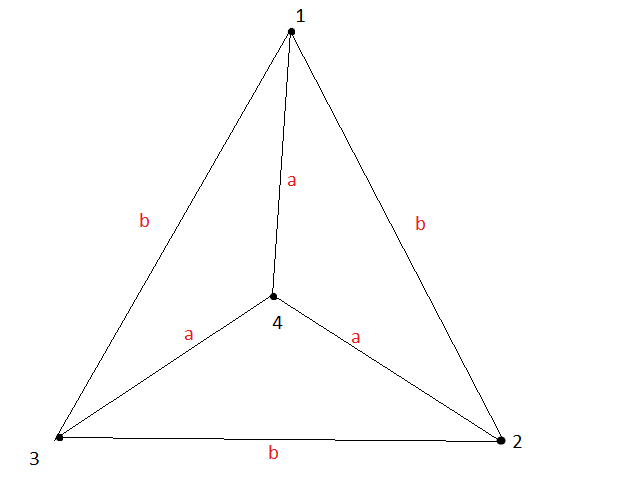
\includegraphics[scale=.5]{images/exemple_borne}
\caption{Exemple de graphe sur lequel la borne de la 2-approximation est atteinte}
\label{exborne}
\end{figure}
 

On remarque donc que $First\_solution$ est bien une solution admissible vu que tous les terminaux seront ajoutés et connectés 2 à 2. On peut prouver que cet algorithme donne une deux approximation\footnote{pour une démonstration de ce principe voir https://people.eecs.berkeley.edu/~luca/cs261/lecture02.pdf}. Je ne ferai pas ici la démonstration mais me contenterai de présenter un cas ou la borne est atteinte : (voir figure \ref{exborne} On voit que notre algorithme va choisir les arêtes $(1,2)$ $(2,3)$ et $(1,3)$ sans passer par le nœud $4$ alors que l'optimum (si $2a<b$ est de choisir les arêtes $(1,4)$ $(2,4)$ et $(3,4)$. Quand b tend vers 2a le ratio entre les deux tends vers 2.



\subsection{Une anecdote d'optimisation}
Une petite anecdote pour bien rappeler le concept de "avant de trouver des stratégies efficaces déjà optimise ton code" :
Après avoir remarqué que mon algorithme d'optimisation était particulièrement lent (voir même ne marchait pas du tout sur les très larges instances) j'ai remarqué que pour chaque tour de boucle pour les couples de terminaux je calculais le plus court chemin entre ces deux terminaux. Ce qui revenait à faire $O(t^2)$ Dijkstra (avec $t$ le nombre de terminaux).  Il suffit en réalité de calculer pour chaque $t_1$ son plus court chemin à tous les points du graphe (ce qui ne coûte qu'un seul Dijkstra) et d'utiliser le résultat pour tous les $t_2$ pour le plus court chemin entre $t_1$ et $t_2$. Cela améliore grandement les performances de notre algorithme, évidemment particulièrement quand le nombre de terminaux et fort. 

\begin{tabular}{|c|c|c|c|c|c|}
\hline 
temps de calcul (en s) & non optimisé & optimisé & nœuds & arêtes & terminaux \\ 
\hline 
instance 039 & 3,31 & 0,143 & 320 & 640 & 80 \\ 
\hline 
instance 001 & 1,09 & 0,525 & 6405 & 10454 & 16 \\ 
\hline 
instance 019 & 177,8 & 13,4 & 38307 & 71546 & 58 \\ 
\hline 
instance 143 & $>3600$   & 16,1  & 2676 & 3894 & 1000 \\
\hline 
\end{tabular} 

\section{Notion de voisin}


\subsection{Présentation du précédent papier}
Par la suite la plupart de nos optimisation se baseront sur une notion de "voisin" des solutions. Il faut évidemment que ces "voisins" soit proche d'un point de vue de score face au problème. Cette proximité dans le cas de graphes comme les notre sera logiquement proche d'une métrique comparant les ensembles de sommets. Cependant comme expliqué dans ce rapport, il n'est pas suffisant de regarder les ensembles de d’arêtes directement. L'ajout ou la suppression d’arête ne suffit pas. On a donc implémenté un nouveau "modificateur" : l'ajout de chemin. 
Pour résumer nous avons quatre "modificateurs" d'une solution courante :
\begin{itemize}   
\item[\textbf{L'addition  d’arêtes : }] on ajoute un certain nombre d'arêtes "voisine" de notre graphe. C'est à dire d'arêtes dont au moins un des nœuds fait déjà partie de la solution. En effet sinon on risque de souvent rajouter des arêtes complètement déconnectées de notre graphe qui n'ont que très peu D’Intérêt.
\item[\textbf{La suppression d’arêtes : }] on supprime des arêtes qui laisse notre solution admissible. Après cette suppression on recalcule les composantes connexes et on ne garde que la composante connexe contenant tous les terminaux (ils sont tous dans la même car la solution reste faisable) 
\item[\textbf{Ajouter un chemin: }] On choisit aléatoirement (uniformément) deux nœuds de notre solution actuelle et on ajoute toutes les arêtes et tous les nœuds d'un plus court chemin les reliant.
\item[\textbf{Clear : }] on nettoie la solution, c'est à dire que tant que c'est possible on supprime des arêtes qui laisse la solution admissible.
\end{itemize}

\subsection{Choix de voisin}

On a de nombreux choix pour comment parcourir notre espace de solution. Nous appellerons "modifications élémentaires" les trois premières modifications décrites plus haut. Le clear sera généralement utilisé en fin de création d'une solution. J'ai implémenté 3 différentes manière d'obtenir un voisin. Toutes dépendent d'un radius $ r$ de recherche qui va correspondre au nombre de modifications élémentaires qu'on va s'autoriser. 

La fonction voisin renvoie une solution : la solution qu'on lui donne à laquelle on a appliqué $r$ fois une des fonctions $one\_step\_search$ décrites ci dessous, puis applique clean sur cette solution.

\subsubsection{Version 1}

Cf one\_step\_search() dans le fichier local\_search.

La version la plus simple qui consiste à tirer aléatoirement l'une des trois modification élémentaire et l'appliquer. Cette méthode est relativement efficace. Seul problème le coup de la suppression d'arête est (dans mon implémentation) très élevée. En effet il faut pour chaque arêtes de la solution en cours calculer toutes les composantes connexes de la solution privée de cette arête. Après calcul il était évident que cette modification élémentaire était largement plus coûteuse en pratique que les autres modifications élémentaires. D’où l'idée de la seconde version.

\begin{algorithm}[H]
\SetAlgoLined
\KwData{graph, terminals, solution}
\KwResult{voisin de solution}
r = random()\;
\If{$r<1/3$}
{
	edge\_addition(graph, solution)\;
}
\If{$r\geq 1/3$ et $r<2/3$}
{
	add\_random\_path(graph, solution)\;
}
\If{$r\geq 2/3$}
{
	edge\_suppresion(solution, terminals)\;
}
\Return(solution)\;
\caption{version\_1}
\end{algorithm}


\begin{tabular}{|c|c|c|c|c|c|c|}
\hline 
temps (en s) & ajout & ajout path & suppression & nœuds & arêtes & terminaux  \\ 
\hline 
instance 001 & 0,03 & 0,01 & 6,63 & 320 & 640 & 80 \\ 
\hline 
instance 039 & 0,07 & 0,01 & 58,34 & 6405 & 10454 & 16 \\ 
\hline 
instance  19 & 0,32 & 1,70 & 1052 & 38307 & 71546 & 58 \\
\hline 
instance  143 & 0,17 & 0,03 & 423,4 & 2676 & 3894 & 1000 \\ 
\hline 
\end{tabular} 

\subsubsection{Version 2}
Cf one\_step\_search\_v2() dans le fichier local\_search.

Cette version voulait s'affranchir du problème du coût de suppression... Elle s'est donc complètement affranchie de la suppression d'arête. En effet cette version est environs 5 fois plus rapide mais comme décrit ci dessous, ses résultats sont légèrement plus faibles on peut donc vouloir garder la notion de suppression d'arêtes.

\begin{algorithm}[H]
\SetAlgoLined
\KwData{graph, terminals, solution}
\KwResult{voisin de solution}
r = random()\;
\If{$r<1/2$}
{
	edge\_addition(graph, solution)\;
}
\If{$r\geq 1/2$}
{
	add\_random\_path(graph, solution)\;
}
\Return(solution)\;
\caption{version\_2}
\end{algorithm}

\subsubsection{Version 3}

Cf one\_step\_search\_v3() dans le fichier local\_search.

Cette ultime version n'est pas spécialement plus rapide (bien que légèrement) que la précédente. Elle est légèrement moins randomisée. En effet on remarque que faire des suppression a tour de bras avant d'avoir modifié notre solution ne semble pas pertinent. On va donc forcer une modification d'ajout (aléatoirement ajout d'arêtes ou de chemin) puis une suppression, puis à nouveau une modification d'ajout. Ceci donne de meilleurs résultats que la version 1 entièrement randomisée. Un idéal serait sans doute une version 4 a mi chemin entre les deux, forçant avec haute probabilité des additions puis des suppressions puis des additions mais laissant un léger aléatoire. On peut pour certains tests choisir aléatoirement entre appliquer la version 1 et la version 3. 

\begin{algorithm}[H]
\SetAlgoLined
\KwData{graph, terminals, solution}
\KwResult{voisin de solution}
solution = version\_2(graph, terminals,solution)\;
edge\_suppresion(solution, terminals)\;
solution = version\_2(graph, terminals,solution)\;
\Return(solution)\;
\caption{version\_3}
\end{algorithm}


\subsubsection{Comparaison des versions}

La figure \ref{comparelocal} nous présente un exemple de test sur une instance (instance 039) de la fonction local\_search\_only\_better (décrite dans la partie suivante) avec 1000 itérations. Le temps d’exécution est relativement long (environs 25 minutes pour la version 1 et 3 et 5 pour la version 2). Les points rouges sont le gain de notre meilleure solution a l'instant $k$ et les points bleus le gain du voisin calculé pour l'instant $k$.

On voit clairement que la version 2 est aussi efficace : convergence légèrement plus lente pour des valeurs équivalentes, convergence finale beaucoup plus haute que les autres versions et gains des solutions visitées bien plus hauts que celles des deux autres. 

Les versions 1 et 3 semblent assez proches, bien que la version 3 semble donner de meilleurs résultats.

\begin{figure}

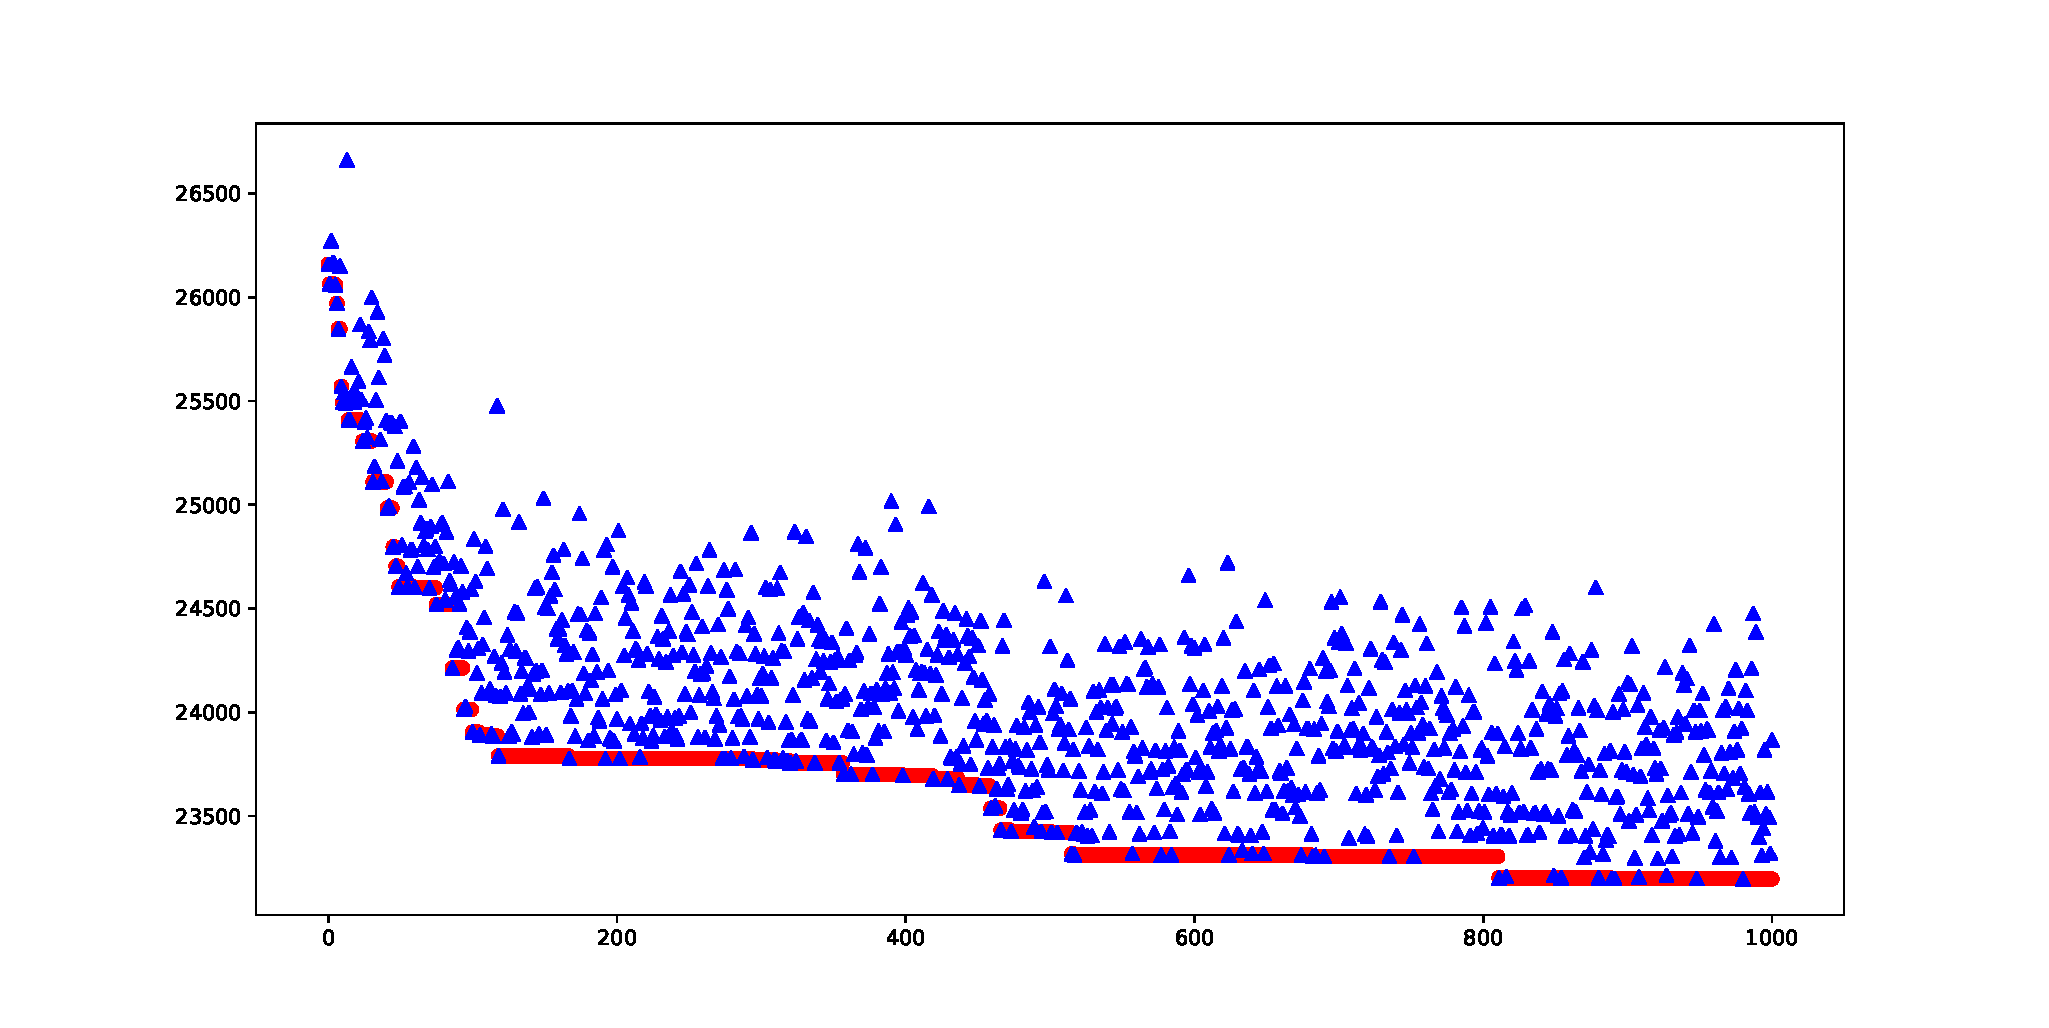
\includegraphics[scale=.4]{images/without_error_1000_v1}
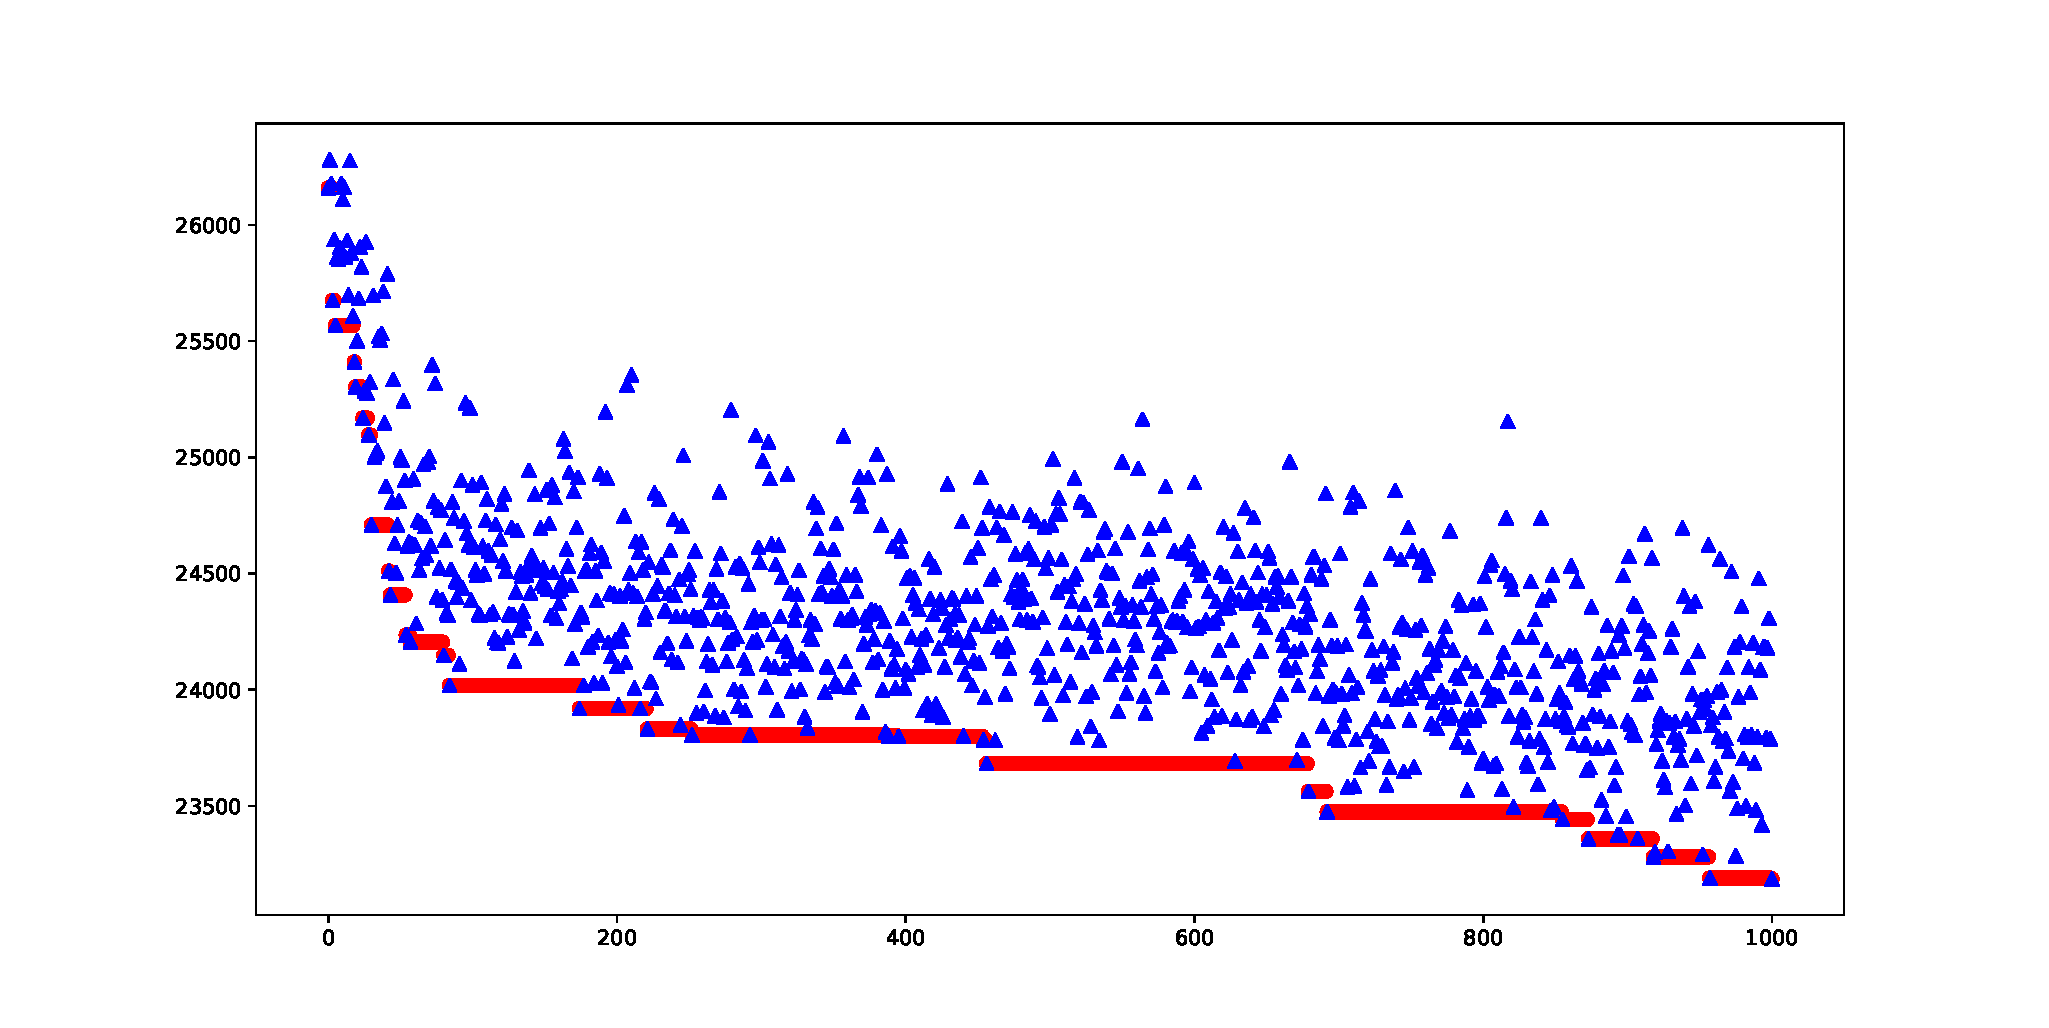
\includegraphics[scale=.4]{images/without_error_1000_v2}
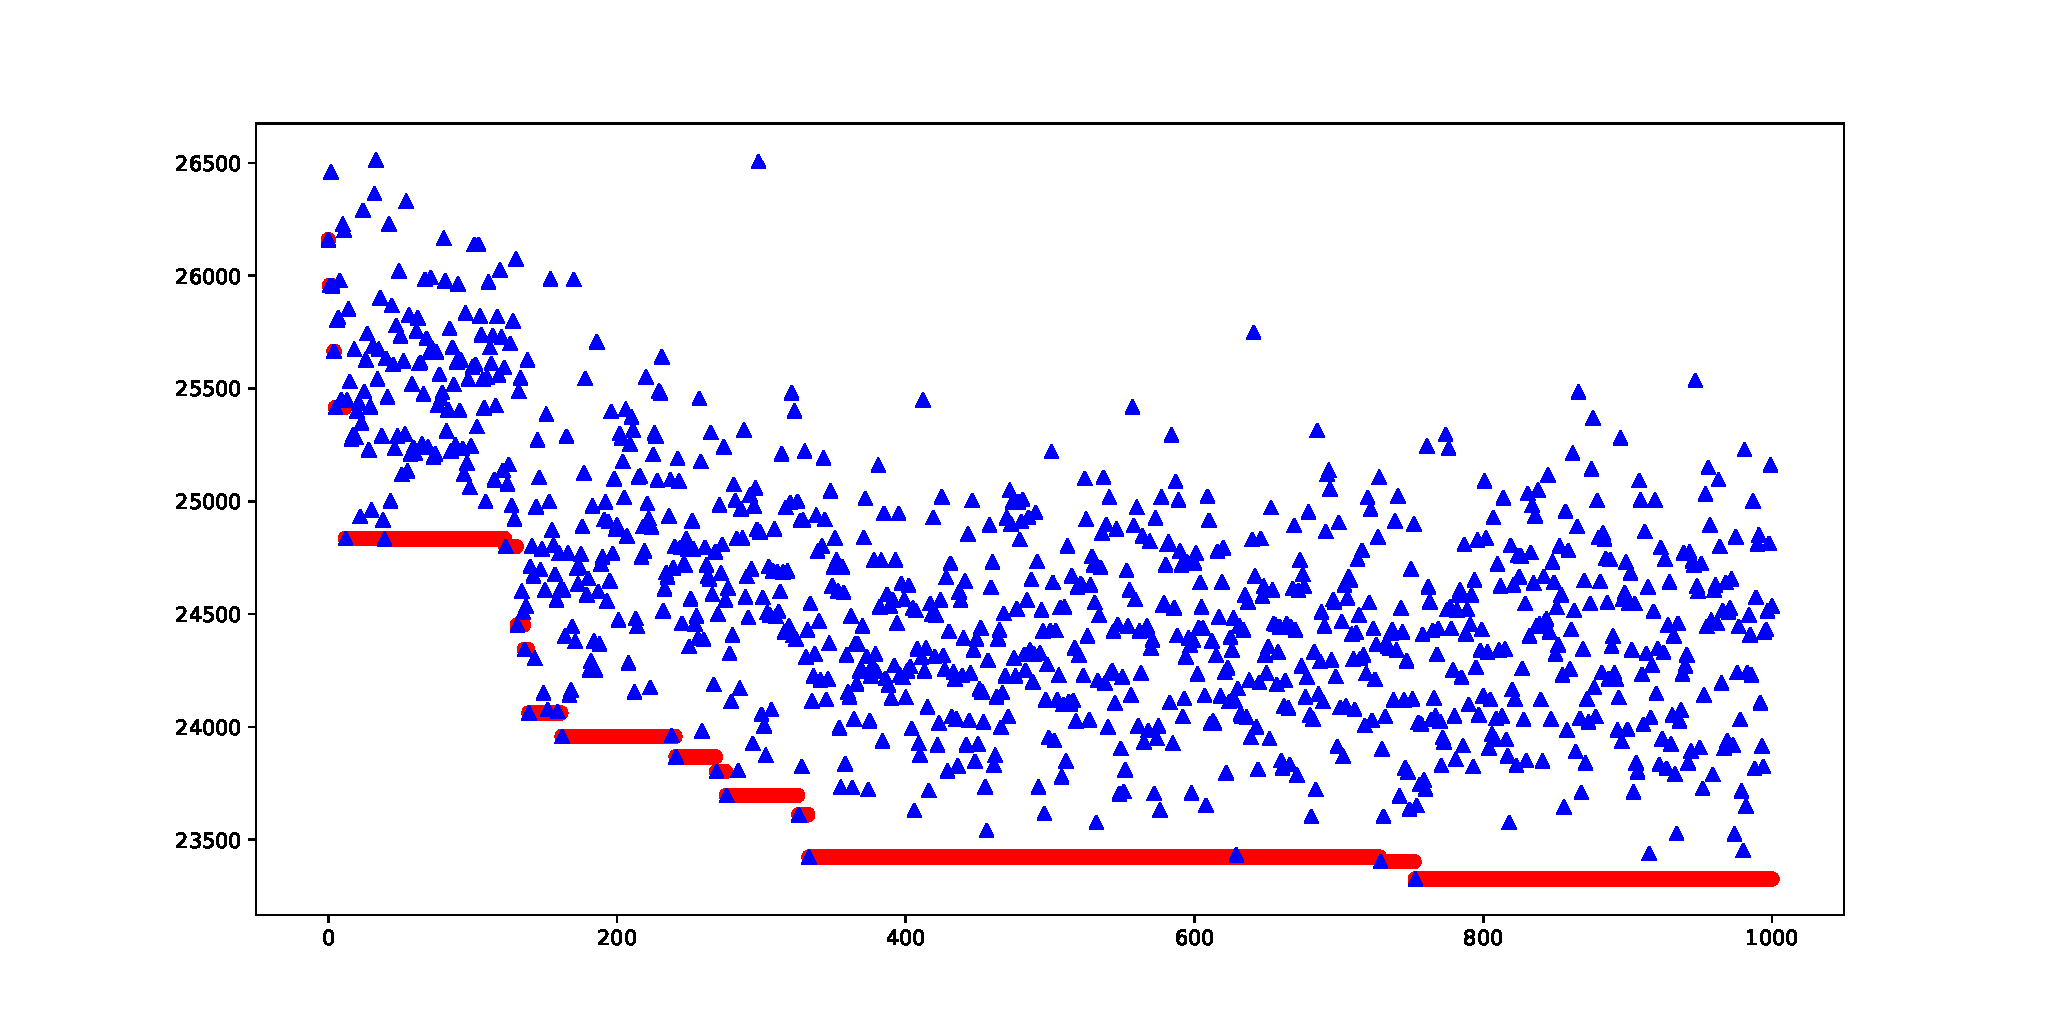
\includegraphics[scale=.4]{images/without_error_1000_v3}
\caption{Dans l'ordre de gauche à droite : version 1, 2, 3}
\label{comparelocal}
\end{figure}


\section{Local Searchs}

On va vouloir parcourir l'ensemble des solutions a la recherche de minimum locaux. Tout le problème de ces parcours est d'arriver a trouver de "bons" minimums locaux, il faut donc en général continuer a trouver un bon trade off entre l'exploration et l'exploitation des points visités.  

\subsection{Sans erreur}


Cf local\_search\_only\_better() dans le fichier simulated\_annealing.

Cette première version est la plus "simple". On n'explore pas du tout de nouvelles parties de notre espace de solution et on se contente de choisir de manière greedy la meilleure solution possible à chaque étape. Nous avons largement utilisé cette fonction pour comparer nos version de choix de voisins. 

\subsection{Avec erreur}

Cf local\_search\_with\_errors() dans le fichier simulated\_annealing.

Cette fois a chaque tour de boucle on s'autorise le choix d'une mauvaise solution. Ce choix est entièrement arbitraire et ne dépend pas de l'erreur que l'on va faire. On pourrait l'améliorer en choisissant une probabilité d'erreur dépendant de l'écart entre la solution actuelle  et de la solution que l'on va peut choisir. La figure \ref{compareerror} montre des exemples avec différentes valeurs pour la probabilité d'exploration.
\begin{figure}
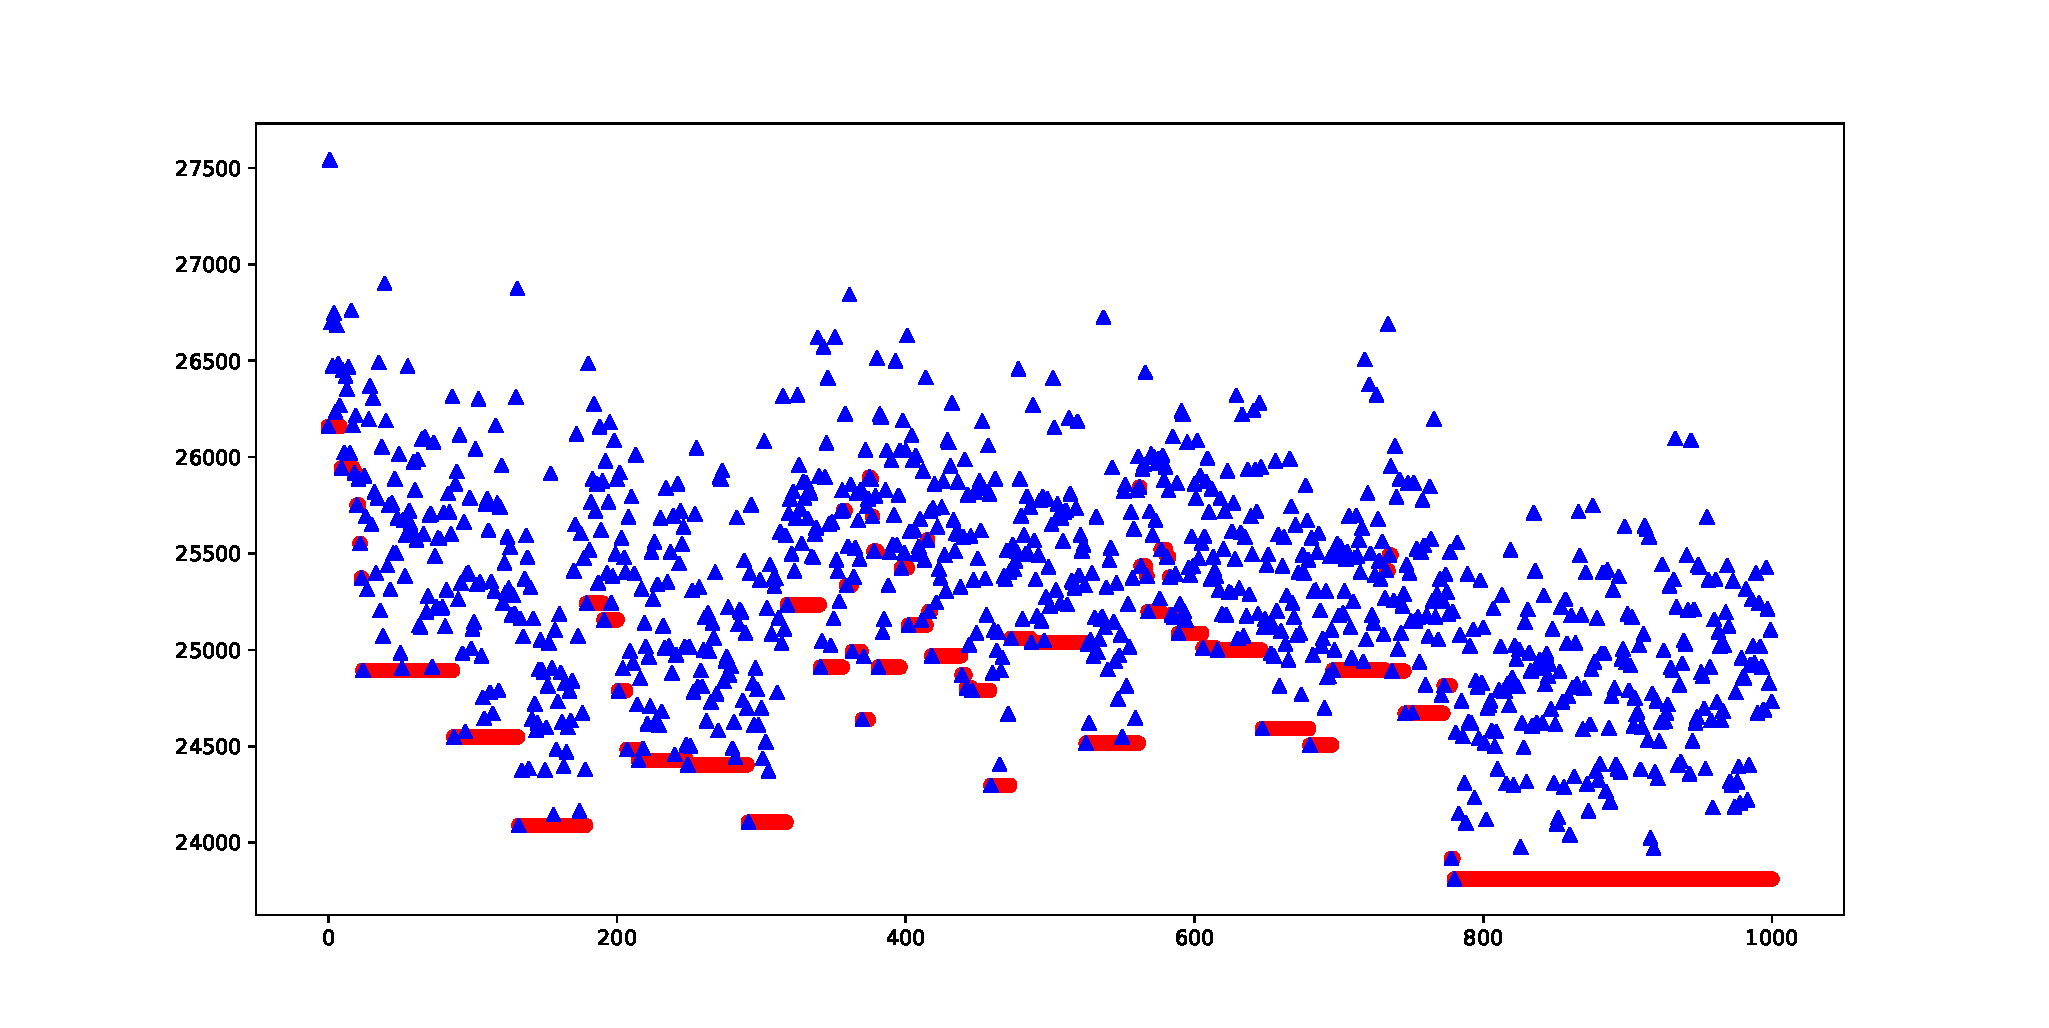
\includegraphics[scale=.35]{images/with_error_01_1000}
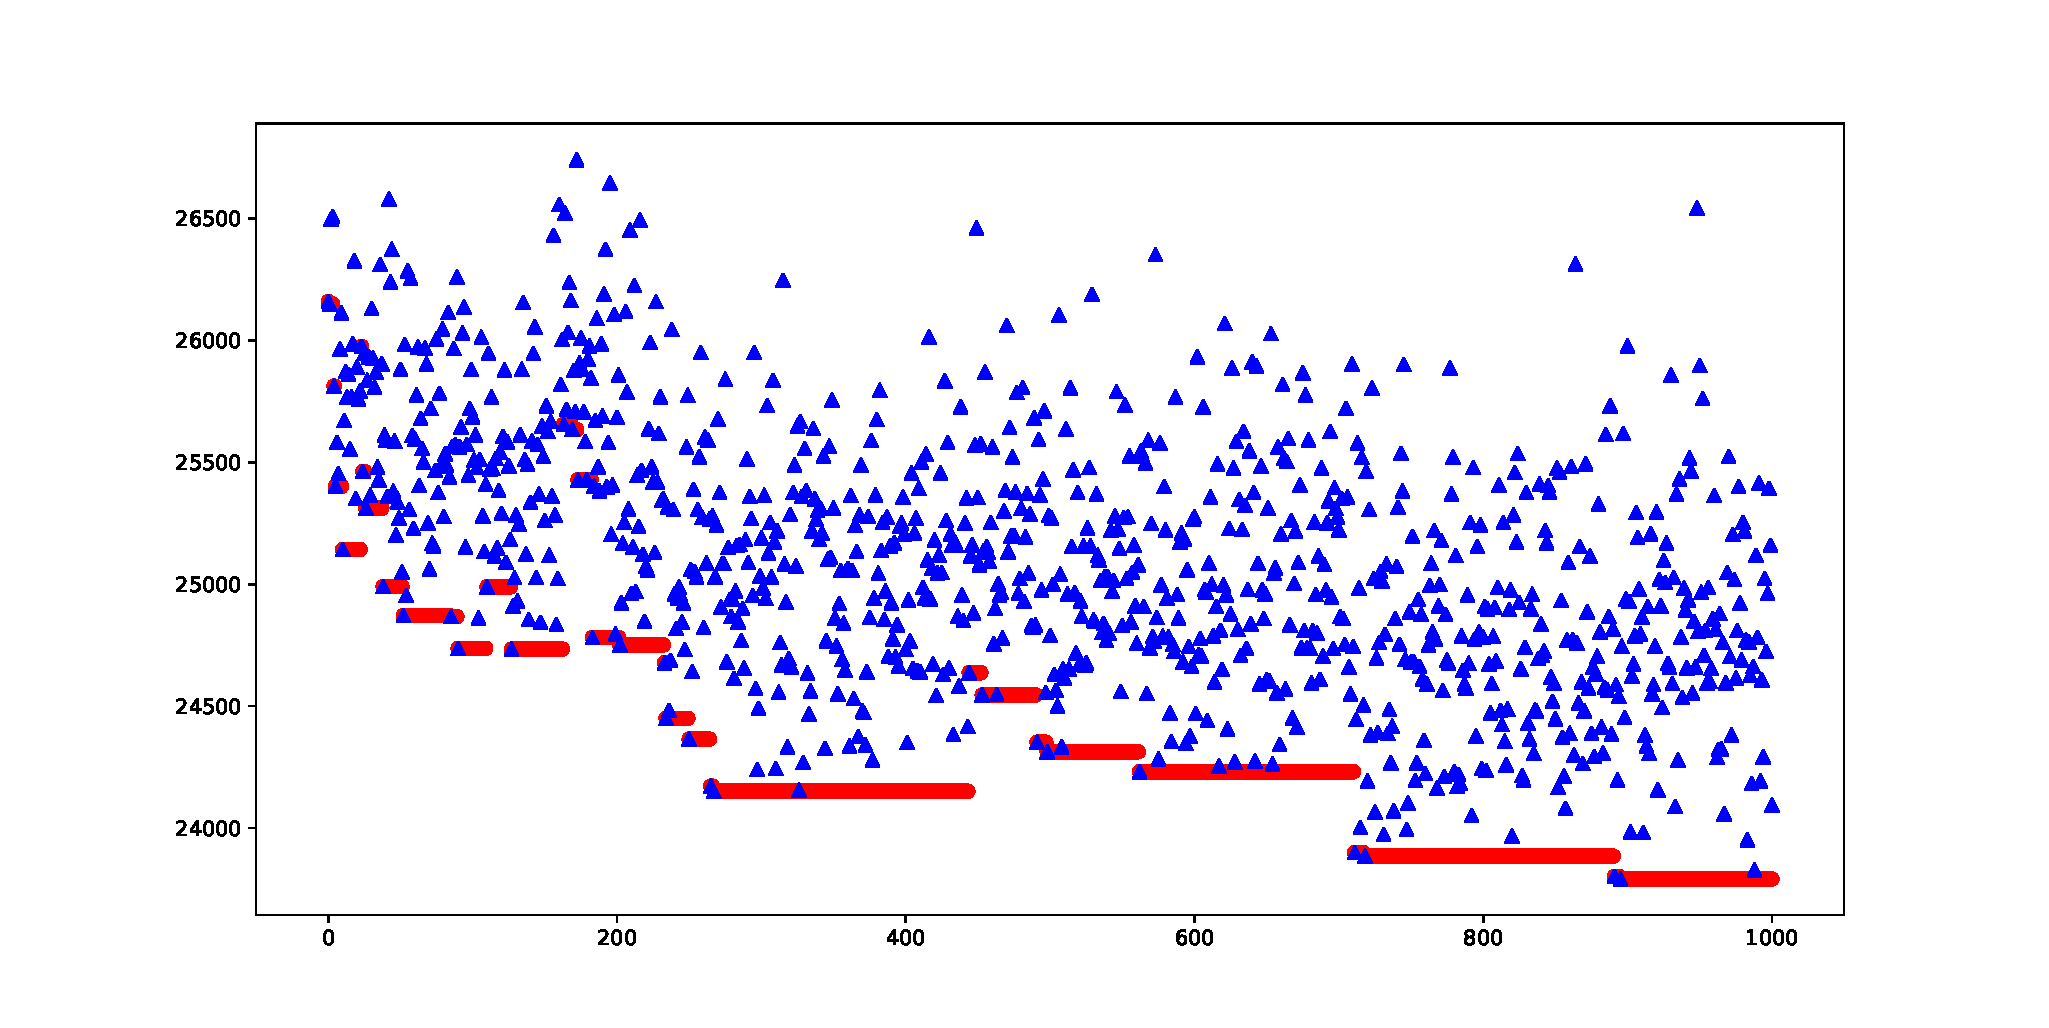
\includegraphics[scale=.35]{images/with_error_005_1000}
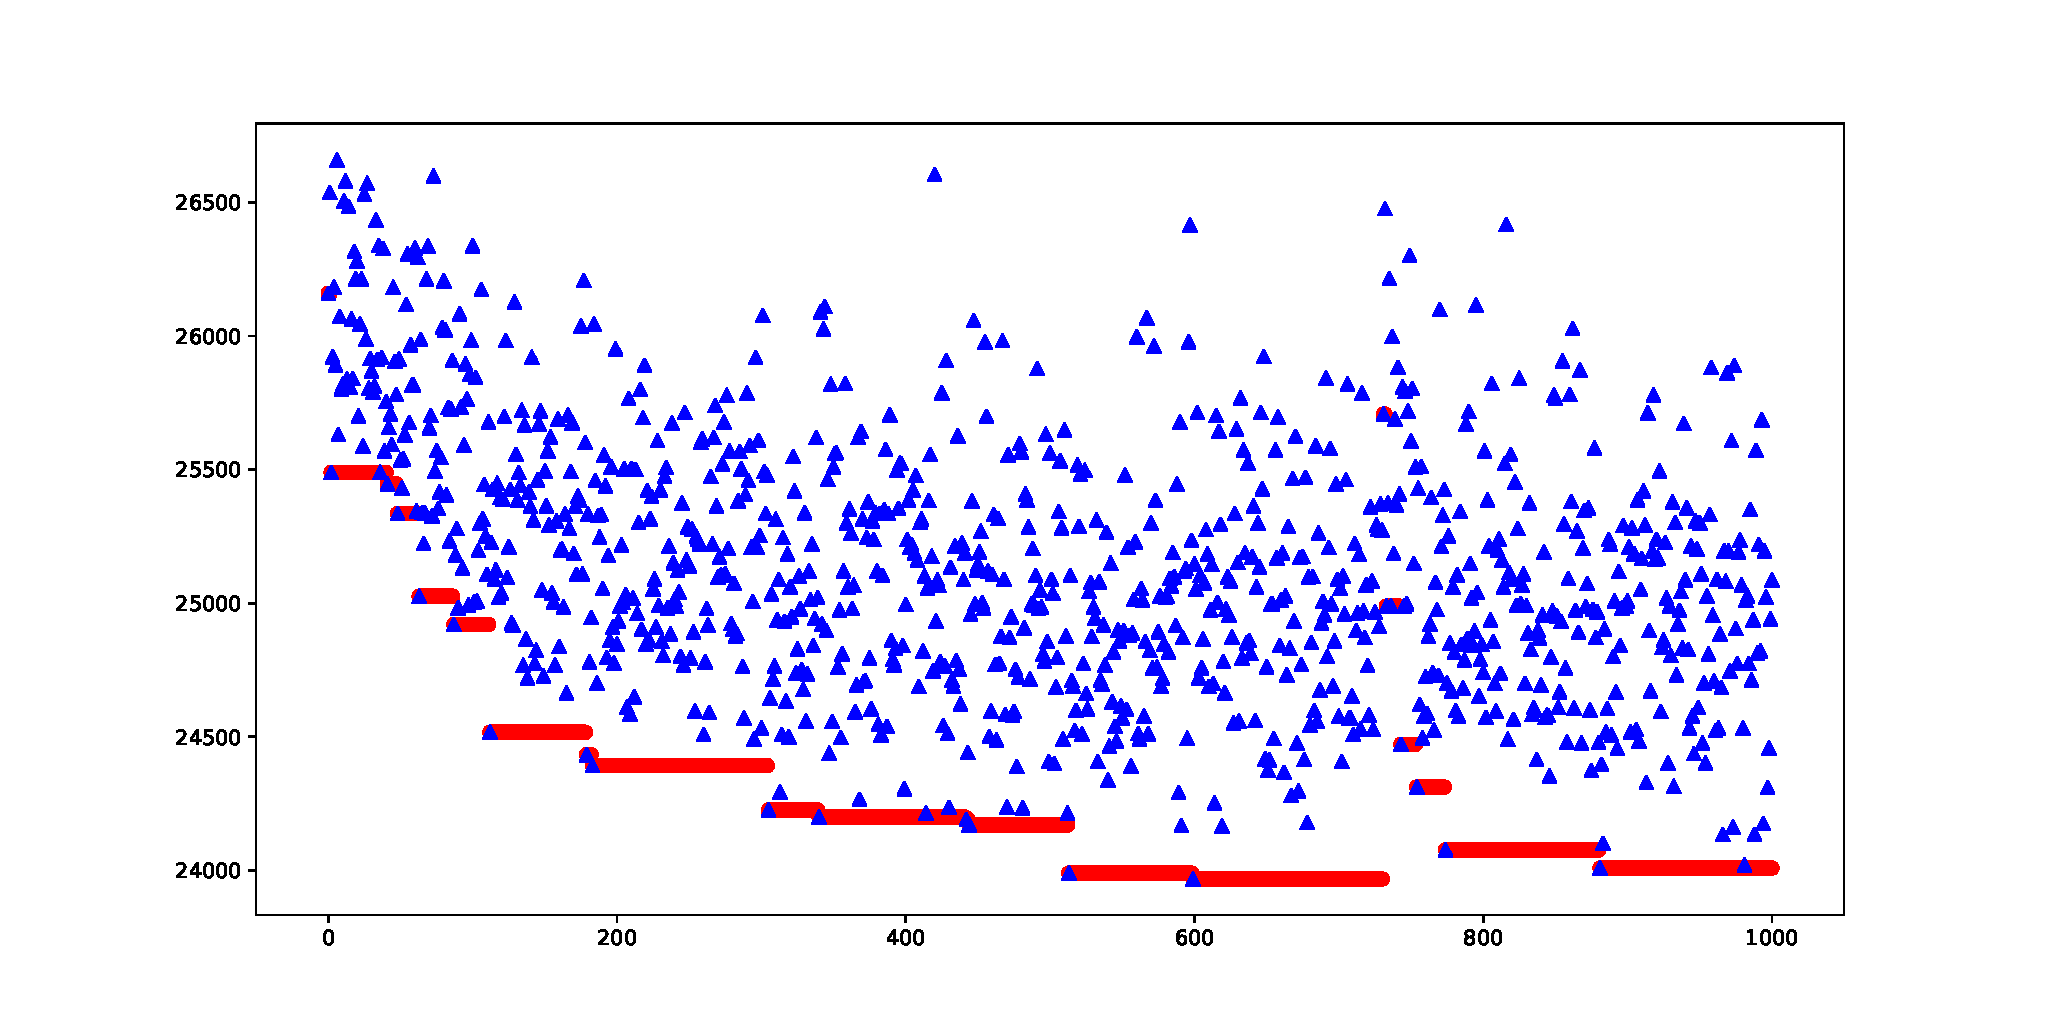
\includegraphics[scale=.35]{images/with_error_001_1000}
\label{compareerror}
\caption{Avec erreur, de haut en bas : erreur en pourcentage 1, 0.5, 0.1}
\end{figure}


\subsection{Recuit simulé}


\subsubsection{Présentation basique}

Le recuit simulé s'appuie sur ce principe de pouvoir choisir une mauvaise solution. Cependant la probabilité d'acceptation de la solution va être indexée sur deux paramètre : le delta entre les deux solutions $\Delta\leq 0$, et une température $T$. La probabilité d'acceptation est généralement la probabilité de Boltzmann : $e^{\frac{\Delta}{T}}$. On remarque donc que plus la température est haute plus la probabilité d'acceptation est forte. L'idée est donc de faire progressivement baisser la température jusqu'à la faire tendre vers 0. Dans un premier temps on s'autorise donc beaucoup d'erreurs assez larges, avant de progressivement se rapprocher d'un algorithme n'acceptant plus aucune erreur. Tout le problème de cet algorithme est le choix de la stratégie pour faire diminuer la température.

\subsubsection{Choix de la température}

J'ai fait le choix d'une stratégie très simple pour la température : simplement choisir $\frac{1}{nb_{iterations}}$ associé parfois d'un correctif multiplicatif pour garder une probabilité décente d'acceptation.

\section{Algorithmes moléculaire}


\subsection{Principe général}

Une autre approche choisit, celle ci moins proche des recherches locale est un type d'algorithme dit biologique appelé algorithme moléculaire. L'idée générale est de maintenir une "population" de solutions (c'est a dire un ensemble de solution). On va ensuite faire évoluer cette population au cours de différentes générations. A chaque génération de nouvelles solutions seront créées et nous ne garderons que les meilleures solutions (ou nous garderons ces solutions du moins avec plus haute probabilité dans le cas de choix randomisés). Le principal problème de cet algorithme est l'ajout de nouvelles solutions

\subsection{Ajouts de solutions à la population }

Nous avons décidé de rester dans un cadre général pour cet algorithme. En effet notre algorithme prend en paramètre une fonction "variation" qui va choisir comment ajouter de nouvelles solutions. Nous avons testé trois principales fonctions de variations qui se basent sur deux principe. Le premier principe est \textbf{le crossover}. L'idée est que si nous avons deux "bonnes" solutions, une combinaison de ces deux solutions donnera encore une "bonne solution". La deuxième approche est juste la \textbf{mutation} des bonnes solutions. La dernière solution est le mix évidemment de ces deux solutions en a la fois qui est généralement le plus utilisé pour les algorithmes moléculaires : à la fois muter des éléments et en fusionner d'autres.



\textbf{Crossover : } on prend en entrée deux solutions $S_1$ et $S_2$. On va créer une nouvelle solution $S_{fils}$ qui sera la fusion des deux solutions pères. On ajoute simplement toutes les arêtes de $S_1$ et $S_2$. On applique ensuite la fonction clean à $S_{fils}$ que l'on renvoie.

\textbf{Mutation : } on utilisera simplement l'une de nos fonctions "voisin" décrites précédemment.


Nous avons donc implémenté trois manières de modifier la population : uniquement du crossover, uniquement de la mutation ou un mix de deux. La figure \ref{compareajout} compare ces différentes manières d'ajouter sur un exemple. Il est logique de voir la stratégie ne faisant que des crossover être très vite limitée : nous n'explorons pas de nouvelles position et au bout de quelques générations on a fait toutes les fusions possible et il n'est plus possible d'améliorer. Même avec des fusions engrainant un peu plus d'aléatoire cette stratégie serait très limitées. La stratégie ne faisant que des mutations reviens en réalité à une forme de local\_search multi threadée.
\begin{figure}
\centering
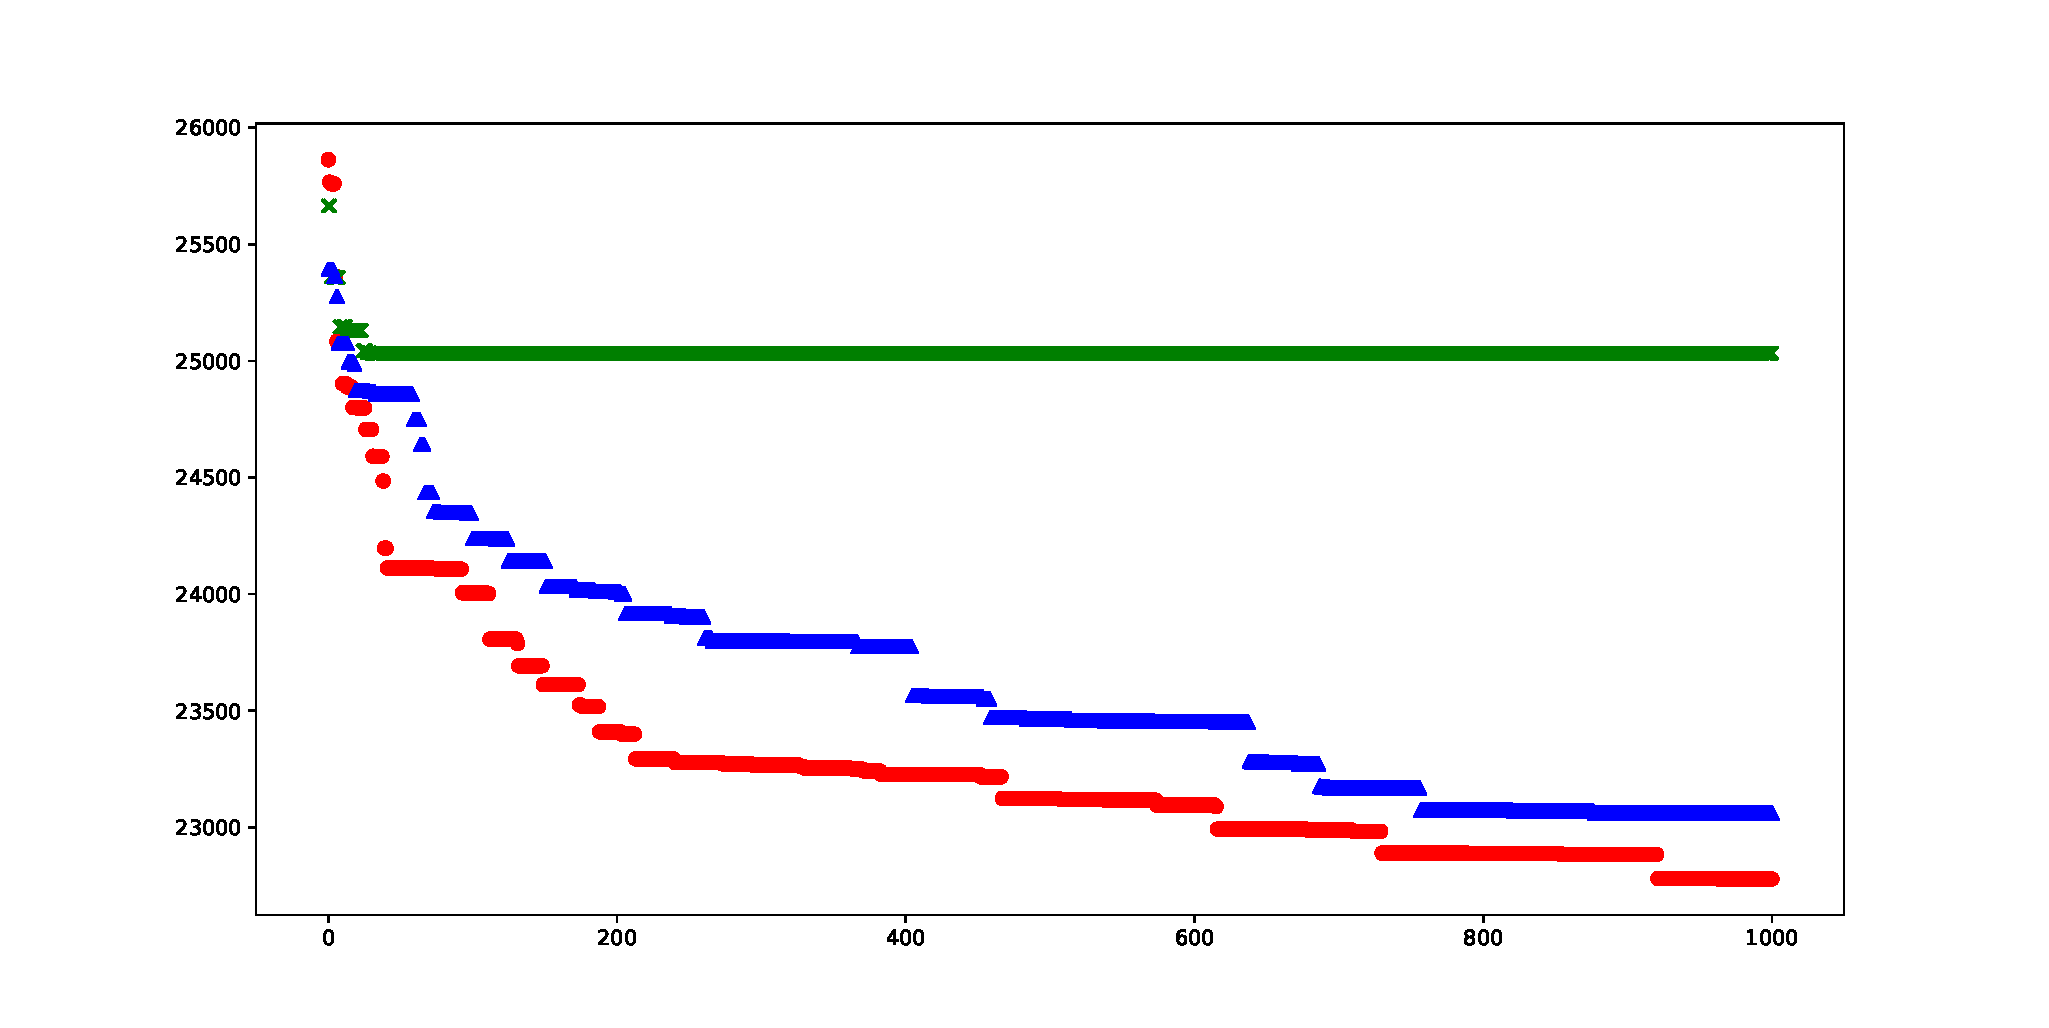
\includegraphics[scale=.4]{images/comparaison_genetic_ajout.pdf}
\caption{Comparaison des différentes stratégies d'ajout. Abscisses : nombre de générations, ordonnées minimum de la génération en cours. 
En vert crossover, rouge mutation, bleu mix de deux}
\label{compareajout}
\end{figure}


Un autre bon indicateur de l'utilité du crossover est le nombre de crossover de la meilleure solution a chaque génération. Nous définissons le nombre de crossover d'une solution par : la somme du nombre de crossover de ses parents +1 si elle issue d'un crossover, son nombre de crossover si elle est issue d'une mutation. Ce nombre est initialisé à 0. La figure \ref{nbcrossover} montre bien que ce nombre suis une loi quasiment (attention les courbes sont en échelle logarithmique), ce qui prouve qu'a chaque génération le crossover à tendance à améliorer la solution. Une première version naïve n'avait tendance qu'à rester aux alentours de 1 ou 3. On voit qu'avec de petites population le nombre de crossover est relativement plus faible mais que la courbe est bien plus croissante du au manque d'exploration de nouvelles solutions, les améliorations doivent se greffer directement sur les solutions déjà bonne. Quand le nombre de génération est plus grand ce nombre fluctue plus 

\begin{figure}
\centering
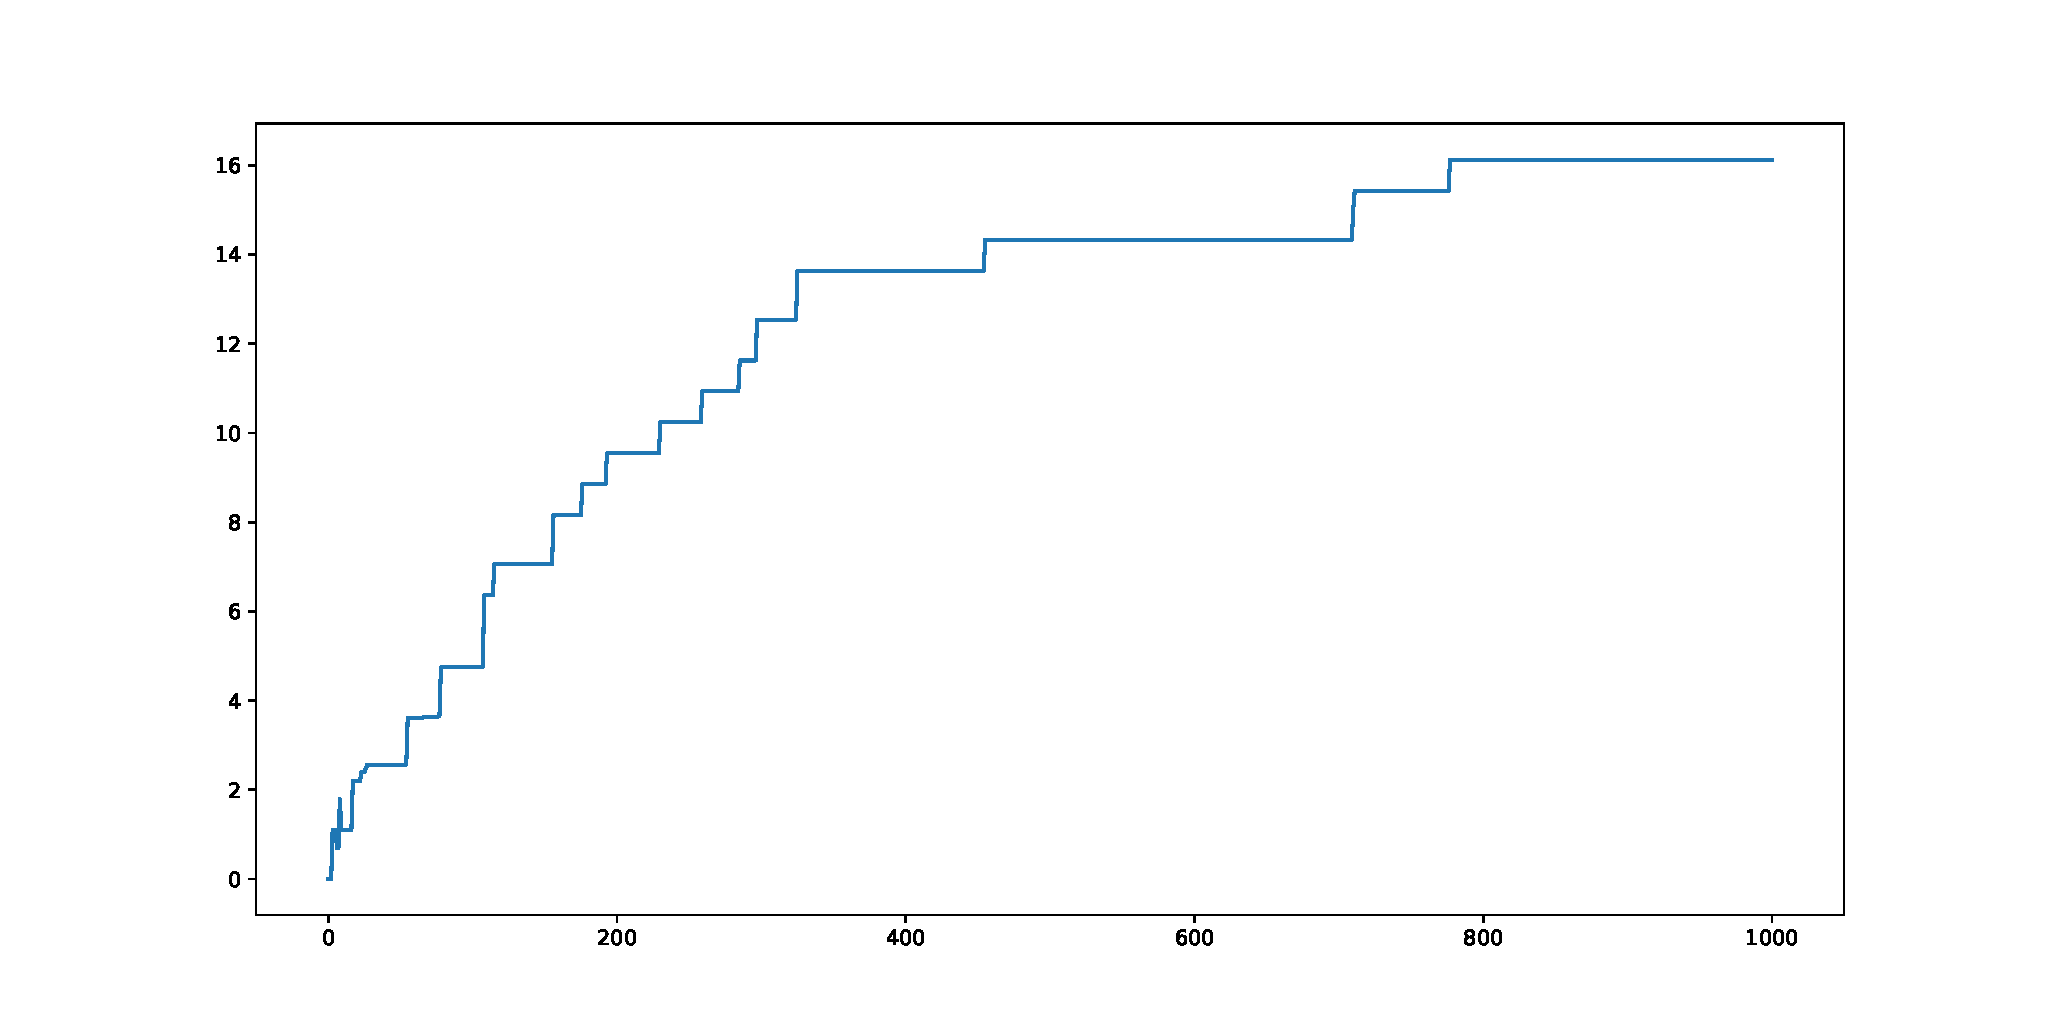
\includegraphics[scale=.4]{images/nombre_fusion_log_5_1000.pdf}
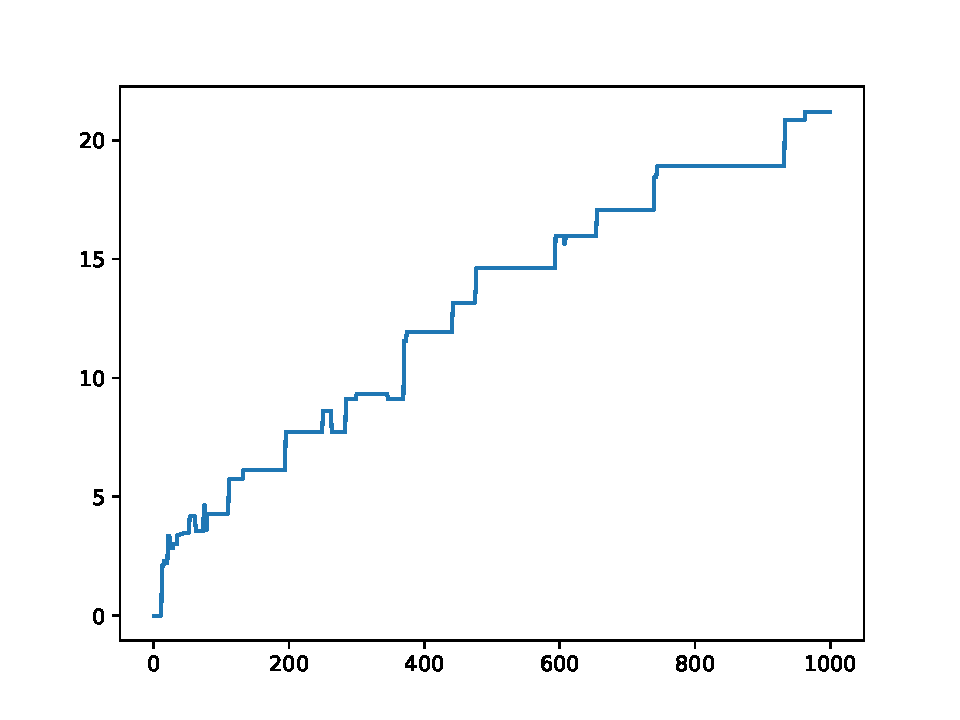
\includegraphics[scale=.6]{images/nombre_fusion_log_30_1000.pdf}
\caption{Logarithme du nombre de crossover au cours 1000 générations. En haut génération de taille 5, en bas de taille 30}
\label{nbcrossover}
\end{figure}

\subsection{Choix de la sélection des survivants}

A chaque génération on choisit un certain nombre de survivants et on élimine les autres solutions. Notre fonction génétique prend en paramètre une fonction de choix des survivants "sélection". 
\begin{itemize}
\item[\textbf{sélection\_elitist\_classic : }] On choisit simplement les meilleures solution de chaque étape
\item[\textbf{sélection\_fitness\_proportional : }] On garde les solutions en fonction de leur ratio par rapport a la moyenne des valeurs des solutions. Pour en choisir $\mu$ on va faire $\mu$ tour de boucle où a chaque tour de boucle on calcule un vecteur qui a chaque solution lui associes (S-coût[sol])/S (ou sol est la solution et S la somme des coûts de toutes les solutions). On normalise le vecteur et cela nous donne la probabilité pour chacune des solutions d'être sélectionnée. 
\item[\textbf{sélection\_Boltzmann: }] On choisit les survivants avec une probabilité de Boltzmann suivant une certaine température fixée
\item[\textbf{sélection\_threshold: }] On accepte les survivants ne dépassant pas le threshold choisit par rapport au minimum de la génération.
\end{itemize}

La figure \ref{compareselection} compare les différentes manière de sélectionner sur un exemple. 

\begin{figure}
\centering
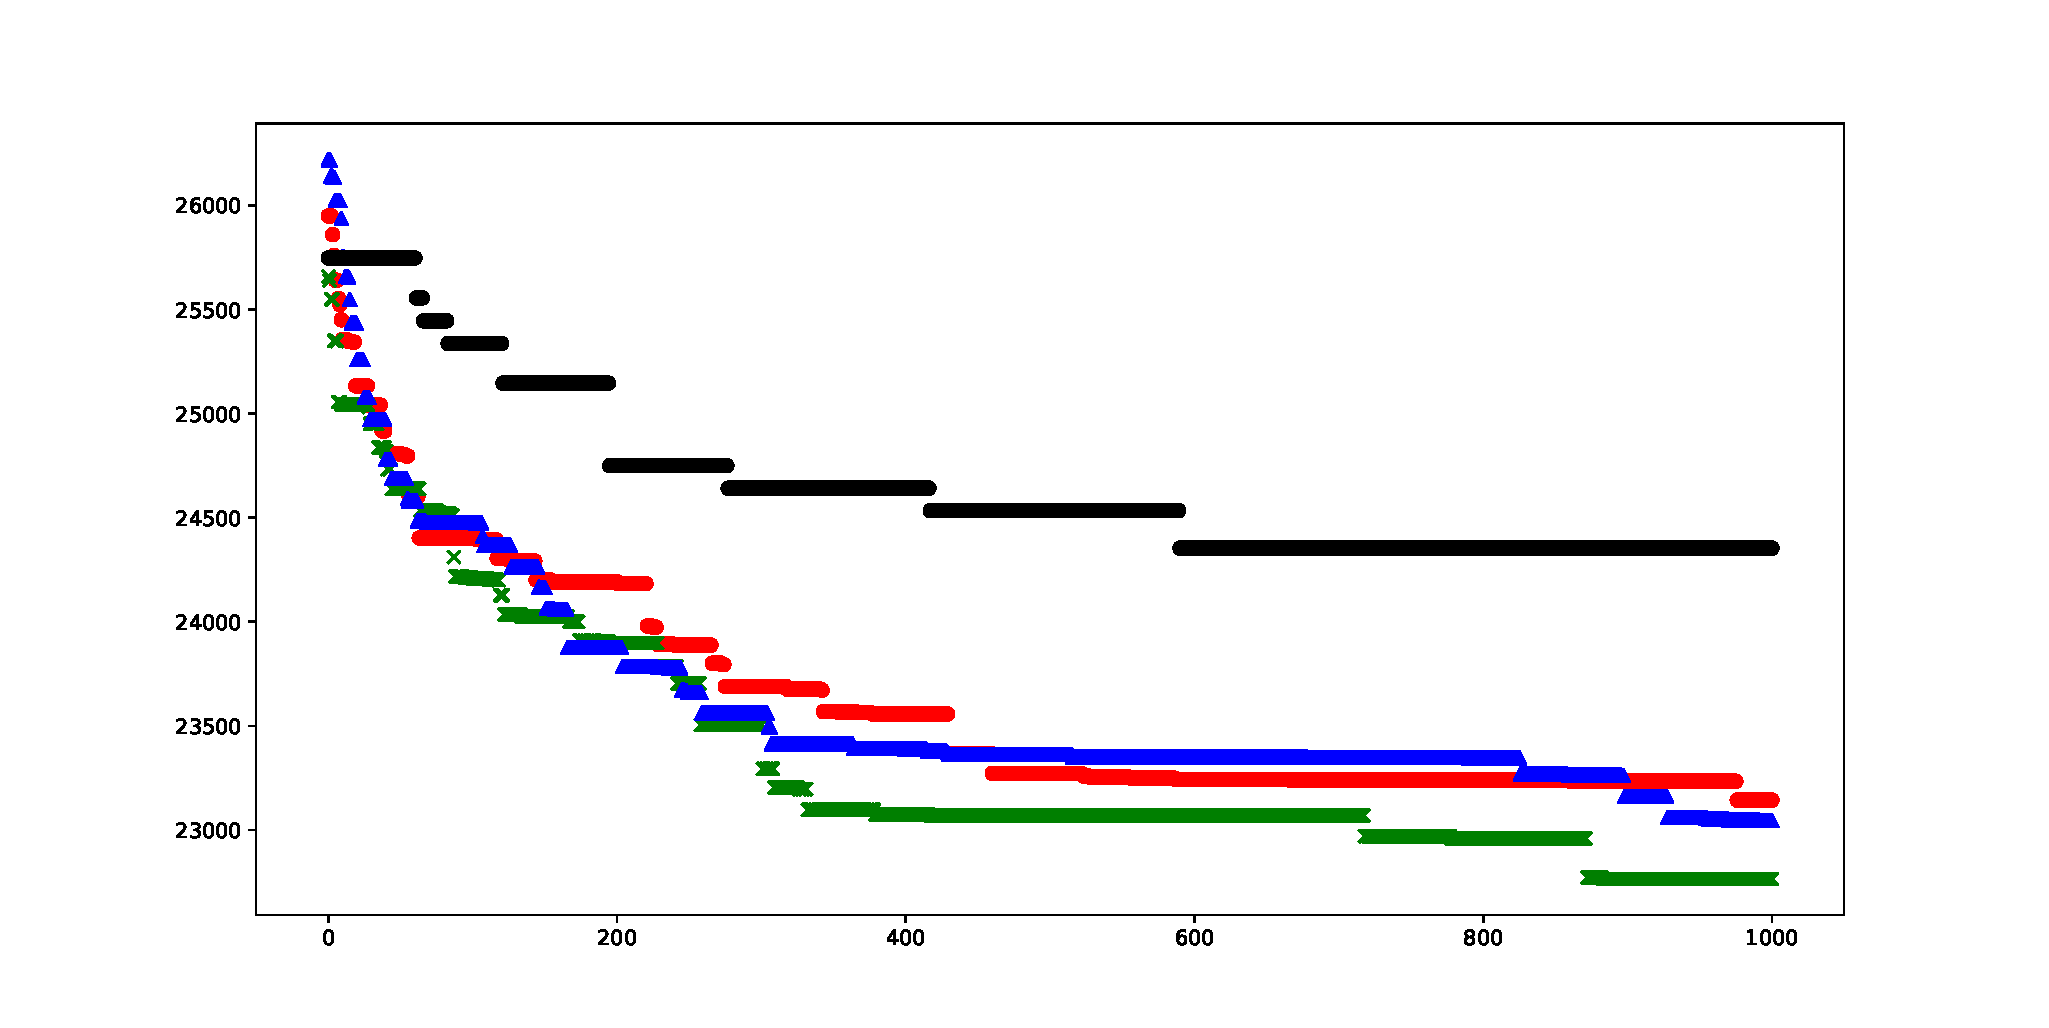
\includegraphics[scale=.4]{images/comparaison_genetic_selection.pdf}
\caption{Comparaison des différentes stratégies de sélection. Abscisses : nombre de générations, ordonnées minimum de la génération en cours. 
En vert classic, rouge offsprings, bleu Boltzmann et noir threshold}
\label{compareselection}
\end{figure}

\section{Comparaisons globales}

Notre dernière comparaison visait à comparer l'algorithme génétiques aux approches locales. Après de nombreux tests l'approche génétique c'est révélée meilleure. Ces comparaisons ont été faites à temps d’exécution équivalente, on ne peut pas comparer le nombre de génération au nombre d'itération des algorithmes locaux (vu que les générations sont composées de plusieurs éléments sur lesquels on peut appliquer des algorithmes locaux). La figure \ref{comparegeneral} compare le meilleur algorithme de recherche locale que nous ayons au meilleur algorithme moléculaire. 


\begin{figure}
\centering
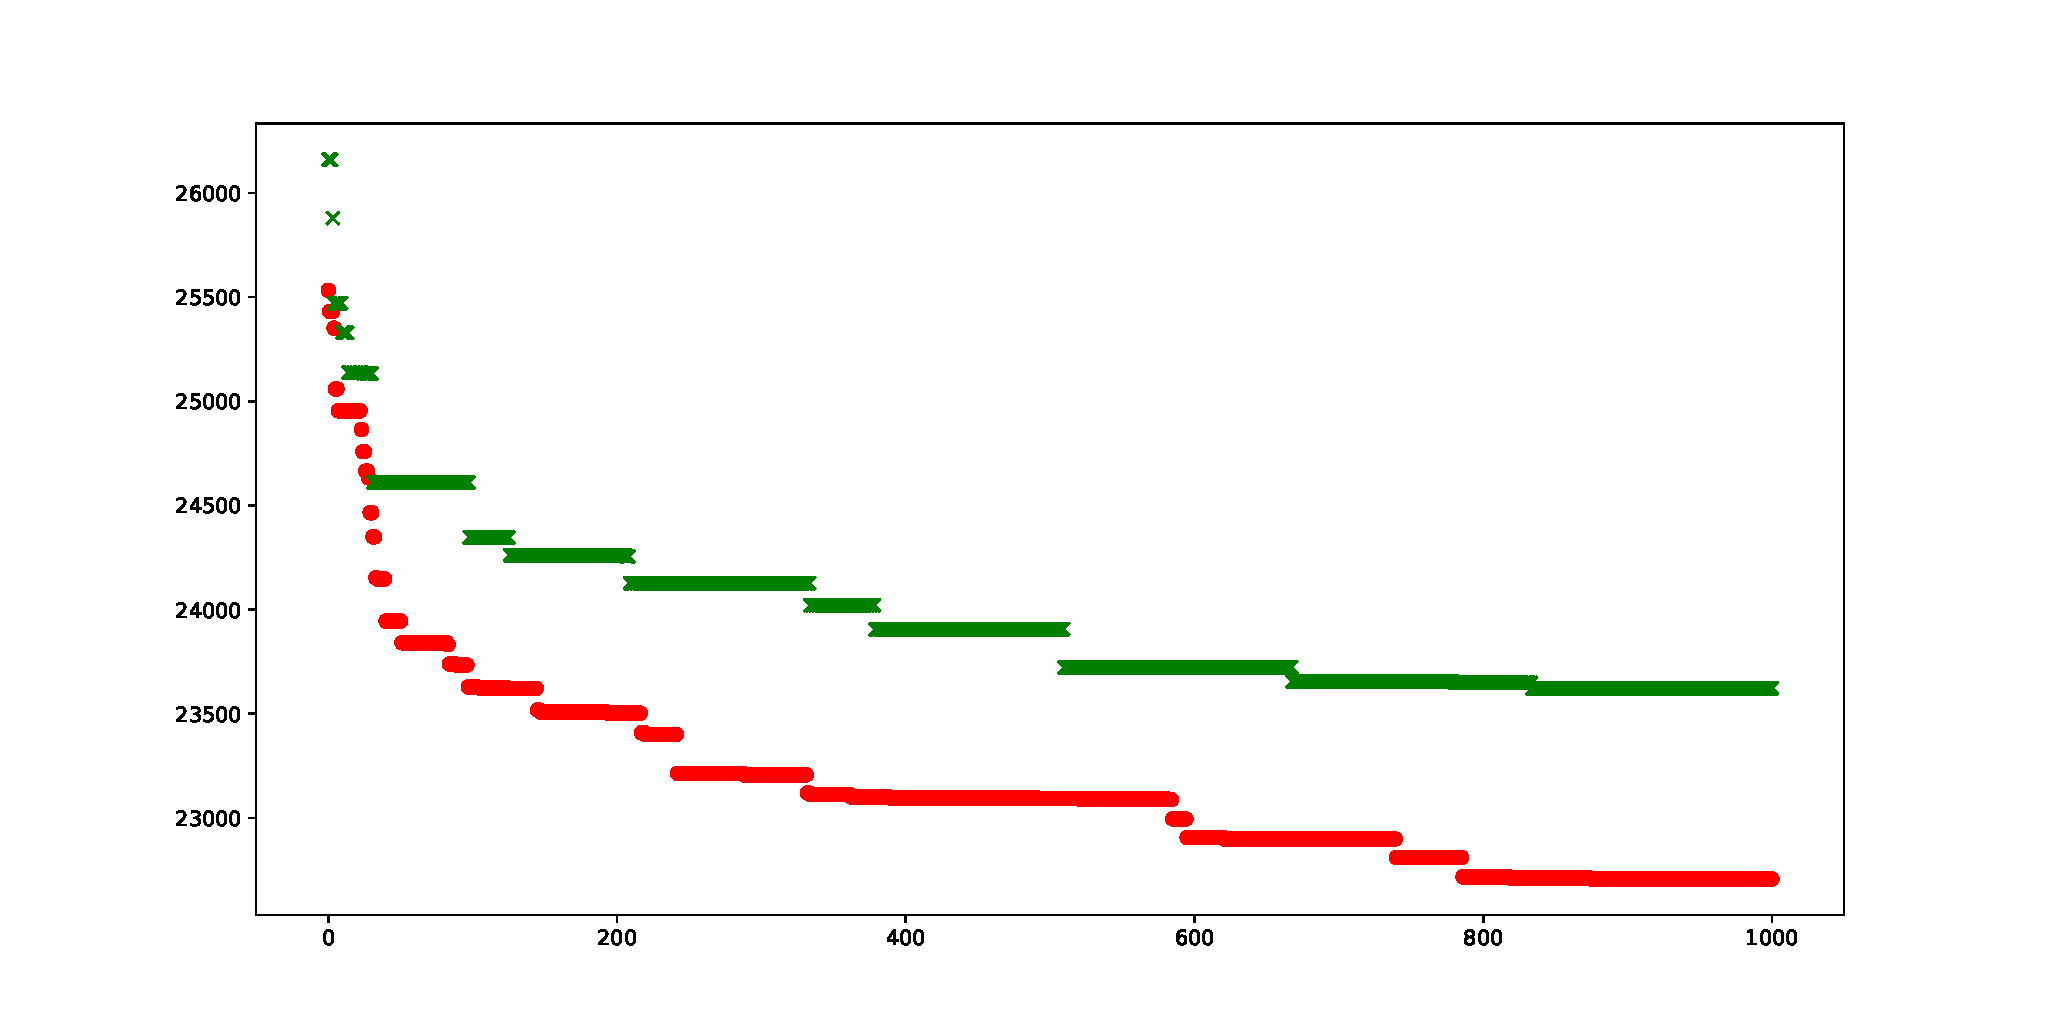
\includegraphics[scale=.4]{images/comparaison_genetic_without_error.pdf}
\caption{Abscisses : temps (normalisé unité non disponible), ordonnées meilleure valeurs au temps donné. En rouge algorithme génétique, en vert algorithme de recherche locale}
\label{comparegeneral}
\end{figure}


\section{Conclusion}

En conclusion les résultats trouvé semblent corrects. Je n'ai malheureusement pas eu le temps de comparer sur le site aux autres personnes mais en comparaison avec d'autres élèves sur l'instance 039 mes résultats semblent tout à fait valable (justification légère mais seule possible pour l'instant). Le fait que le crossover de l'algorithme génétique améliore réellement les solutions est une vraie satisfaction.
 Quelques problèmes d'implémentation m'ont empêches de travailler suffisamment sur le recuit simulé (temps d’exécutions trop longs pour accepter trop d'erreurs).
 
 
\end{document}